\documentclass[a4paper]{scrartcl}

% set geometry of document
\usepackage{geometry} \geometry{ a4paper, left=25mm, right=25mm, top=18mm,
bottom=20mm }

% useful imports
\usepackage{tikz}
\usepackage{extarrows}
\usepackage{proof}
\usepackage{hyperref}
\usepackage[inference]{semantic}
\usepackage{amsmath}
\usepackage{mathrsfs}
\usepackage{stmaryrd}
\usepackage{fancyhdr}
\usepackage[english]{babel}
\usepackage[utf8]{inputenc}
\usepackage{minted}
\usepackage{mdframed}
\usepackage{graphics}

% customize hyperref colors
\usepackage{xcolor}
\definecolor{custom-blue}{RGB}{6,69,173}
\hypersetup{
    colorlinks = true,
    allcolors = custom-blue
}

\begin{document}
\pagestyle{empty}
\begin{center}
\vspace*{30}
\Huge{\sc{Machine Learning in Cybersecurity \\- Midterm Presentation -}}
\\ \\ \\
\Large{Team :flushed:}
\\
\vspace*{100}
\Huge{\sc{Analyzing Apple's NeuralHash.}}
\\
\Large{Q. Zheng, M. Löffler, T. Schneider}
\end{center}
\newpage

\section{Refinded final idea}

Some claims and ideas from our project proposal have to be corrected for them to be realistic and achievable. 
\\
\\
We have claimed that there was no scientific papers similar to our project idea in our initial proposal. Soon this was corrected after we have been pointed to \href{https://arxiv.org/pdf/2111.06628.pdf}{a paper} which analyzes collision-resistance of NeuralHash in a very similar fashion as to what we had planned. 
\\
\\
With this information we want to refocus our project goal a little from producing hash-collisions towards analyzing the robustness of the model. First we want to discuss whether we can leak information about the images by looking at the hash. This can be done by training a second network which classifies hash outputs. We plan to test this on a dataset which specifically is not ImageNet to produce noval results and see if the papers results generalize.  
\\
\\
In an additional second step we want to perform a detection evasion attack. Here we want to see how easy it is to apply minimal pertubations to achieve a maximally different neural hash. This can be done either with gradient based approaches or with simple image manipulations. The second has only been discussed for a limited amount of (reversable) transformations in the paper but it is also of great importance (especially in the use-case of CSAM scans). If there was a simple image filter fooling the network this would render the neural hashing useless.

\section{Progess}

In the following we present our results. Note that we have focused on producing hash-collisions so far.

\subsection{Model extraction}

In a first step we extracted the model together with weight data from a OSX system and converted it to \texttt{.onnx} format. This model is ready to be loaded into our jupyter notebook.

\subsection{Running a POC attack}

We were able to reproduce a proof-of-concept attack obtaining a hash-collision for two seemingly different images by applying rather obtrusive pertubations. The reason for the high pertubation value is that the attack starts reducing pertubation once it could find a true hash collision. On our inputs however this happens rather late, this is further backed by the fact that we reduced the iteration amount by a factor of ten for now. Nonetheless we managed to produce a collision.
\\

\begin{tabular}{c c c}
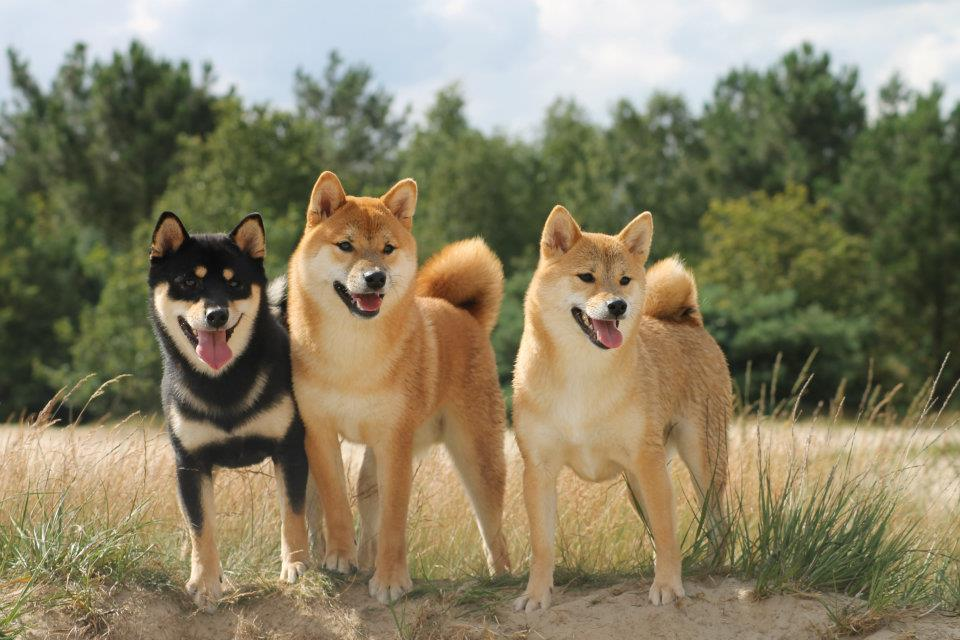
\includegraphics[width=4cm]{doge.jpeg} &
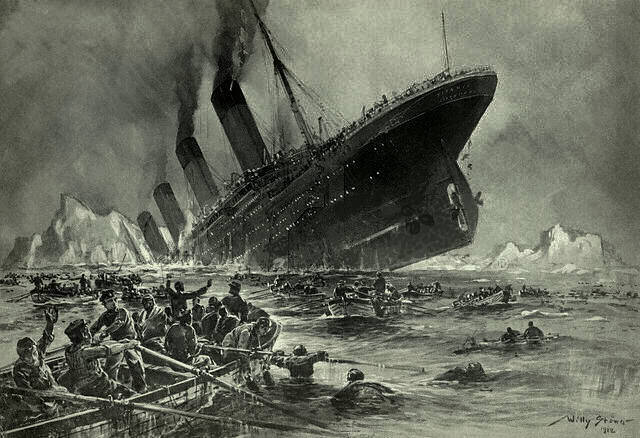
\includegraphics[width=4cm]{titanic.jpeg} &
\includegraphics[width=4cm]{pertubated.png} \\
    4d3032644e122d8c7326cfc9 &
    1ec173f89d10be5300ac0216 &
    1ec173f89d10be5300ac0216
\end{tabular}

\subsection{Challenges}

Obtaining the model and converting it to \texttt{.onnx} was straightforward, however importing it in the notebook was causing cryptic problems for some of us. Producing neural hashs worked out-of-the-box while running the attack required some tweaking. Still it is not running perfectly. First steps would be to swap out distance and loss measures to produce results under smaller pertubation. 

\section{Next Steps}

To successfully refocus the projects goal we need to the following:
\begin{itemize}
	\item Decide on datasets to use (e.g., OpenImages from the projects initial proposal).
	\item Implement a network to classify neural hashes (X) to classes of our dataset (y).
	\item Test to what extend the model can be fooled by proving images pertubated with simple filters.
	\item Collect an present gathered results.
\end{itemize}


\end{document}
